\documentclass[11pt,a4paper]{article}

\usepackage[utf8]{inputenc}
\usepackage[vietnamese,english]{babel}
\usepackage{amsmath,amssymb}
\usepackage{graphicx}
\usepackage{geometry}
\geometry{a4paper, margin=20mm}
\usepackage{booktabs}
\usepackage{float}
\usepackage{hyperref}
\usepackage{xcolor}
\usepackage{fancyhdr}
\usepackage{titlesec}

\hypersetup{
    colorlinks=true,
    linkcolor=blue!70!black,
    citecolor=blue!70!black,
    urlcolor=blue!70!black
}

\pagestyle{fancy}
\fancyhf{}
\rhead{\small \textit{Hệ thống Giám sát \& Điều khiển Phòng Thông minh - STM32F103}}
\lhead{\small \textit{Tài liệu Thiết kế Kiến trúc \& Giải thuật}}
\rfoot{\thepage}

\titleformat{\section}{\large\bfseries\color{blue!60!black}}{\thesection}{1em}{}
\titleformat{\subsection}{\normalsize\bfseries\color{black!80}}{\thesubsection}{1em}{}

\begin{document}
\selectlanguage{vietnamese}

\begin{center}
    {\LARGE \textbf{BÁO CÁO THIẾT KẾ KIẾN TRÚC VÀ GIẢI THUẬT}}\\[2mm]
    {\large \textbf{HỆ THỐNG GIÁM SÁT \& ĐIỀU KHIỂN PHÒNG THÔNG MINH (STM32F103C8T6)}}\\[1mm]
    {\normalsize \textbf{Tài liệu kỹ thuật tổng hợp: Kiến trúc 3-Tier, Máy trạng thái HLSM và Lưu đồ giải thuật Scheduler}}
    \vspace{2mm}
    \hrule height 1pt
\end{center}

\vspace{2mm}

\section{Tổng quan Kiến trúc Hệ thống (3-Tier Layered Architecture)}
Hệ thống được thiết kế theo mô hình kiến trúc phân tầng 3 lớp (3-Tier Architecture) nhằm đáp ứng triệt để các tiêu chuẩn phần mềm nhúng công nghiệp (\textit{stm32f103\_embedded\_rules.md}):
\begin{itemize}
    \item \textbf{Tầng 1 - Phần cứng (Hardware Layer):} Vi điều khiển STM32F103C8T6 (Cortex-M3 @ 72MHz), màn hình màu TFT ILI9341 ($320 \times 240$, SPI1), cảm ứng điện trở XPT2046 (SPI2), 4 nút bấm vật lý (GPIO Pull-up), 4 kênh Relay cách ly quang PC817 (Active-LOW) và 3 cụm cảm biến (DHT22, LDR LM393, PIR AM312).
    \item \textbf{Tầng 2 - Trình điều khiển hệ thống (System Drivers Layer):} Các module \texttt{ili9341.c}, \texttt{xpt2046.c}, \texttt{button.c}, \texttt{font5x7.c} trực tiếp cấu hình thanh ghi / HAL ngoại vi, cung cấp các hàm giao tiếp chuẩn (\texttt{ili9341\_fill\_rect}, \texttt{xpt2046\_read}, \texttt{button\_has\_event}).
    \item \textbf{Tầng 3 - Ứng dụng nghiệp vụ (Application Layer):} Các module \texttt{app\_main.c}, \texttt{display\_manager.c}, \texttt{mode\_control.c}. Tầng này tuân thủ nguyên tắc \textbf{Zero HAL} (tuyệt đối không include HAL hay can thiệp thanh ghi) và \textbf{Zero Float} (100\% dùng số nguyên Fixed-Point).
\end{itemize}

\begin{figure}[H]
    \centering
    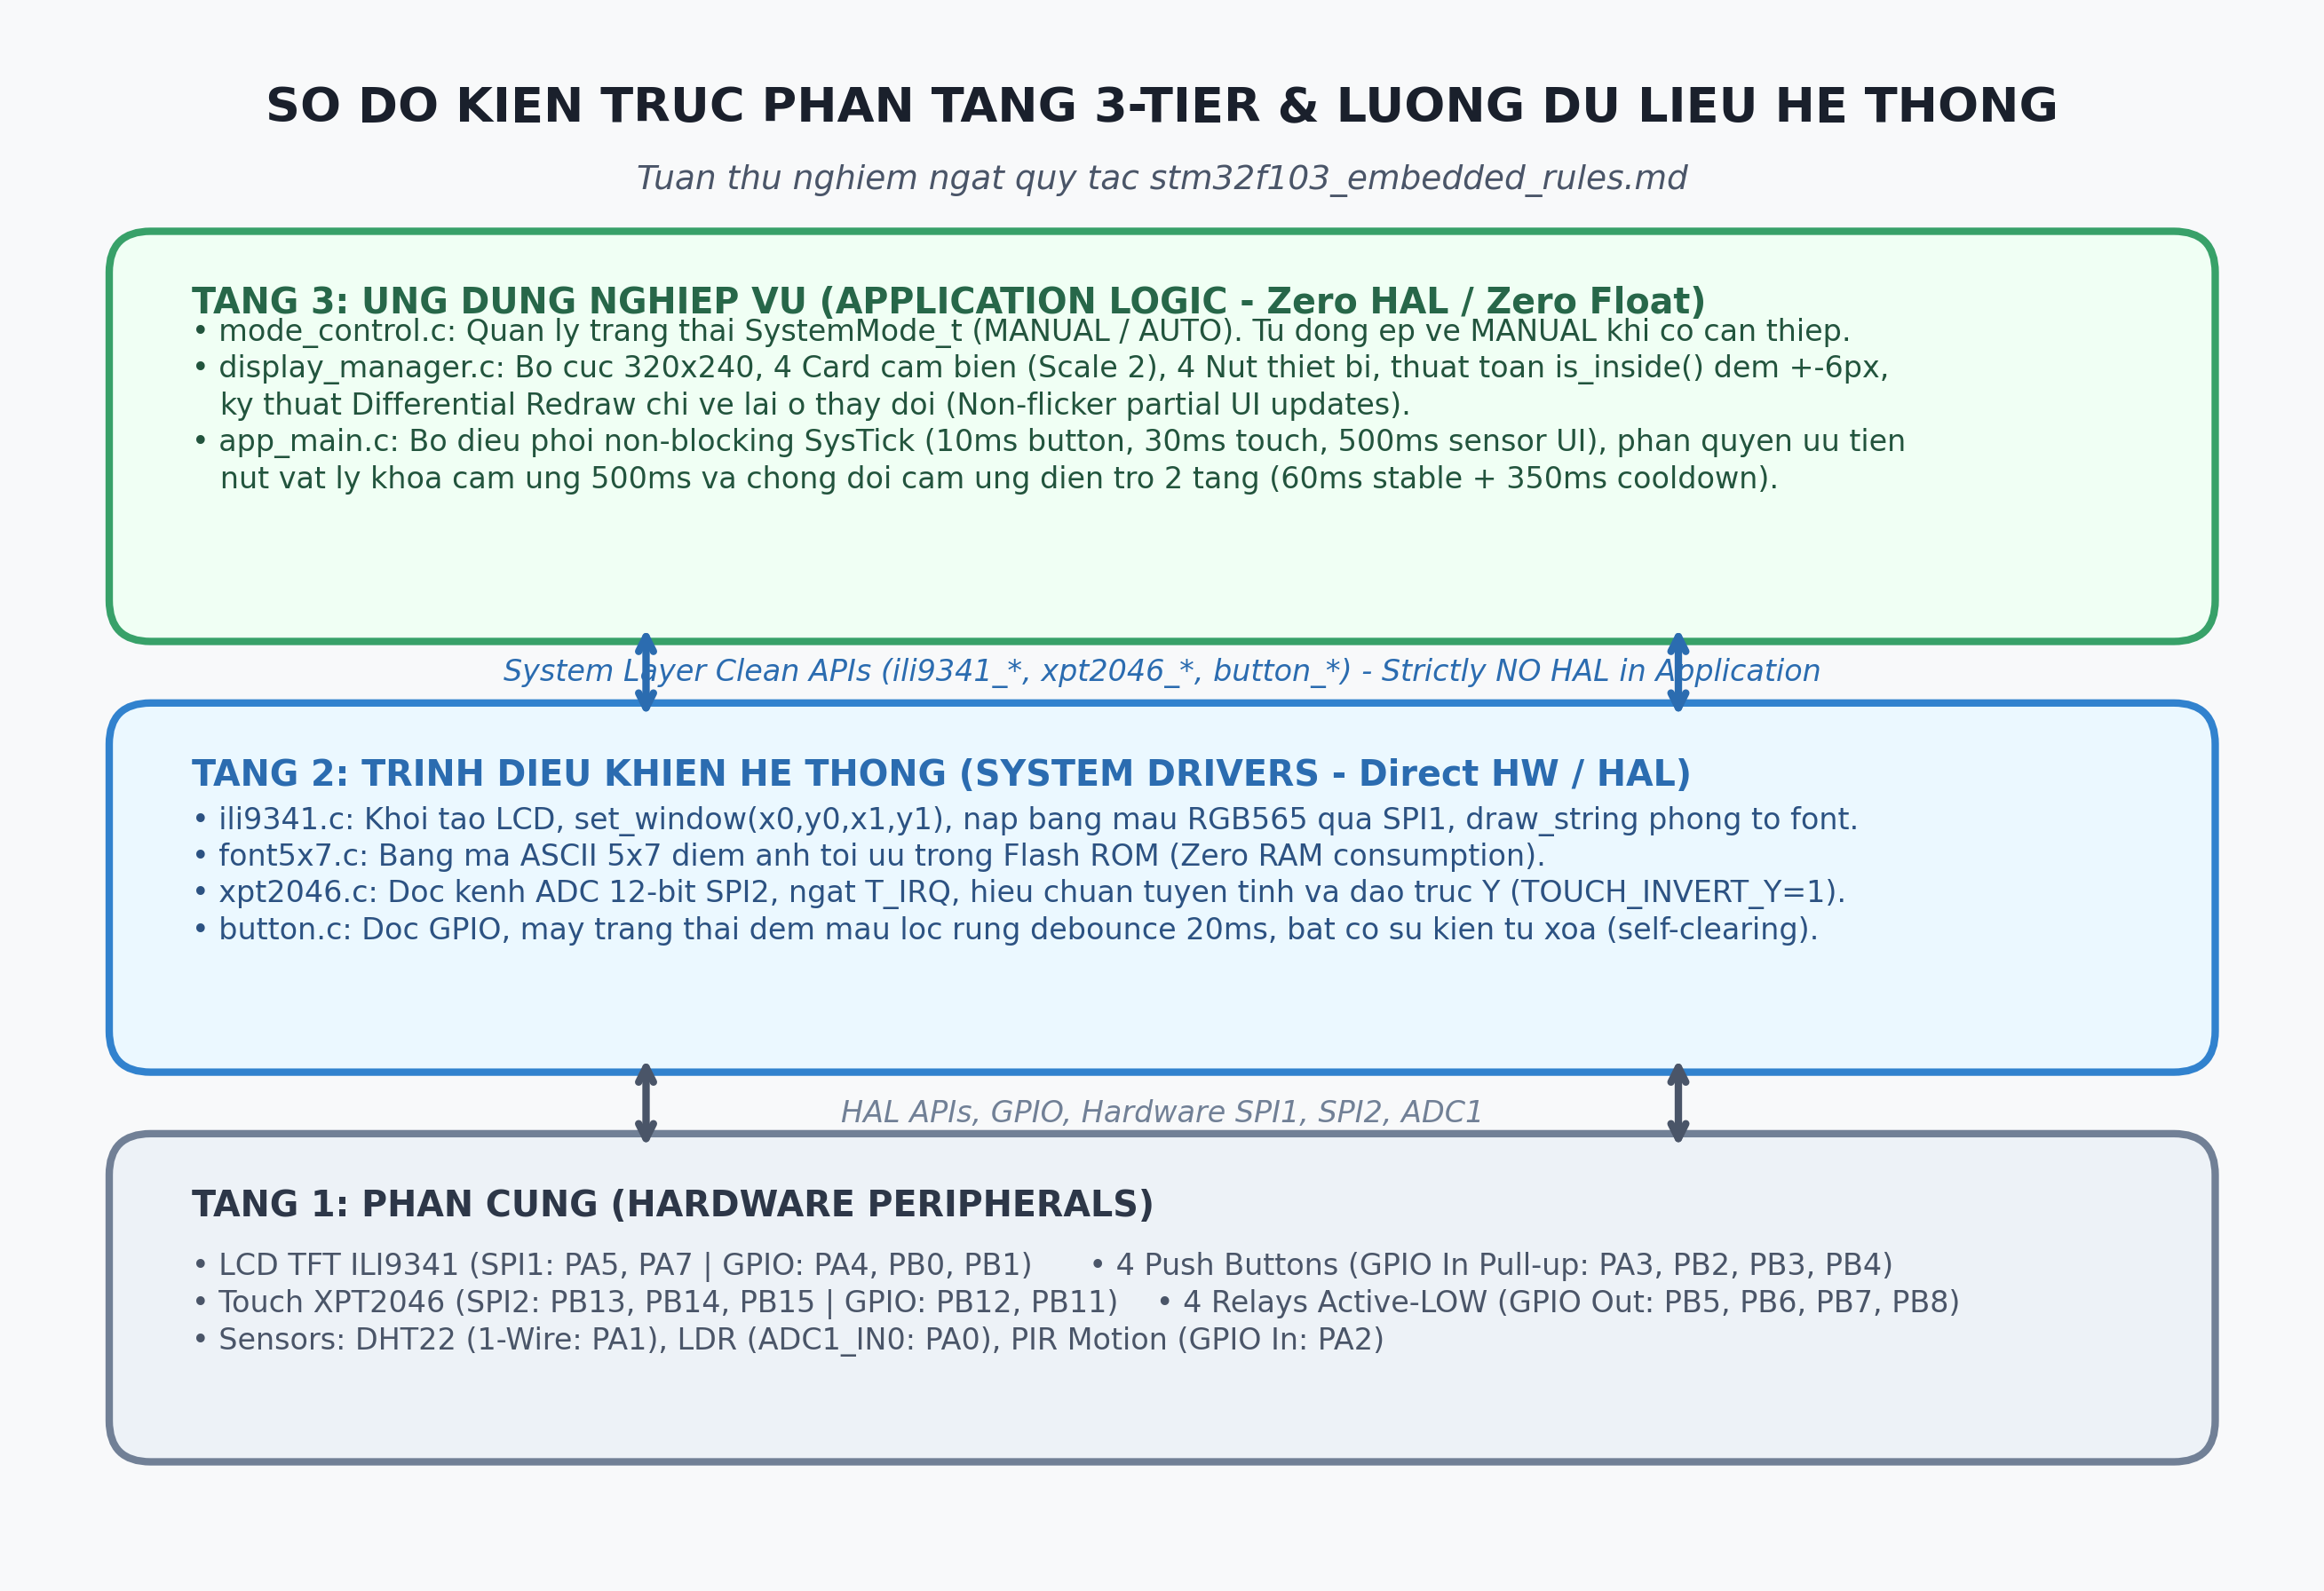
\includegraphics[width=0.95\textwidth]{figures/architecture_interaction.png}
    \caption{Sơ đồ phân tầng kiến trúc 3-Tier và luồng dữ liệu hệ thống}
    \label{fig:arch}
\end{figure}

\section{Máy trạng thái mức cao (HLSM - High-Level State Machine)}
Khác với các lưu đồ tuần tự truyền thống, mô hình HLSM mô tả chính xác sự chuyển đổi giữa hai chế độ hoạt động chính: \textbf{MODE\_MANUAL} và \textbf{MODE\_AUTO}, đồng thời làm nổi bật \textbf{Luật ưu tiên cưỡng bức (Preemption Rule)}.

\begin{figure}[H]
    \centering
    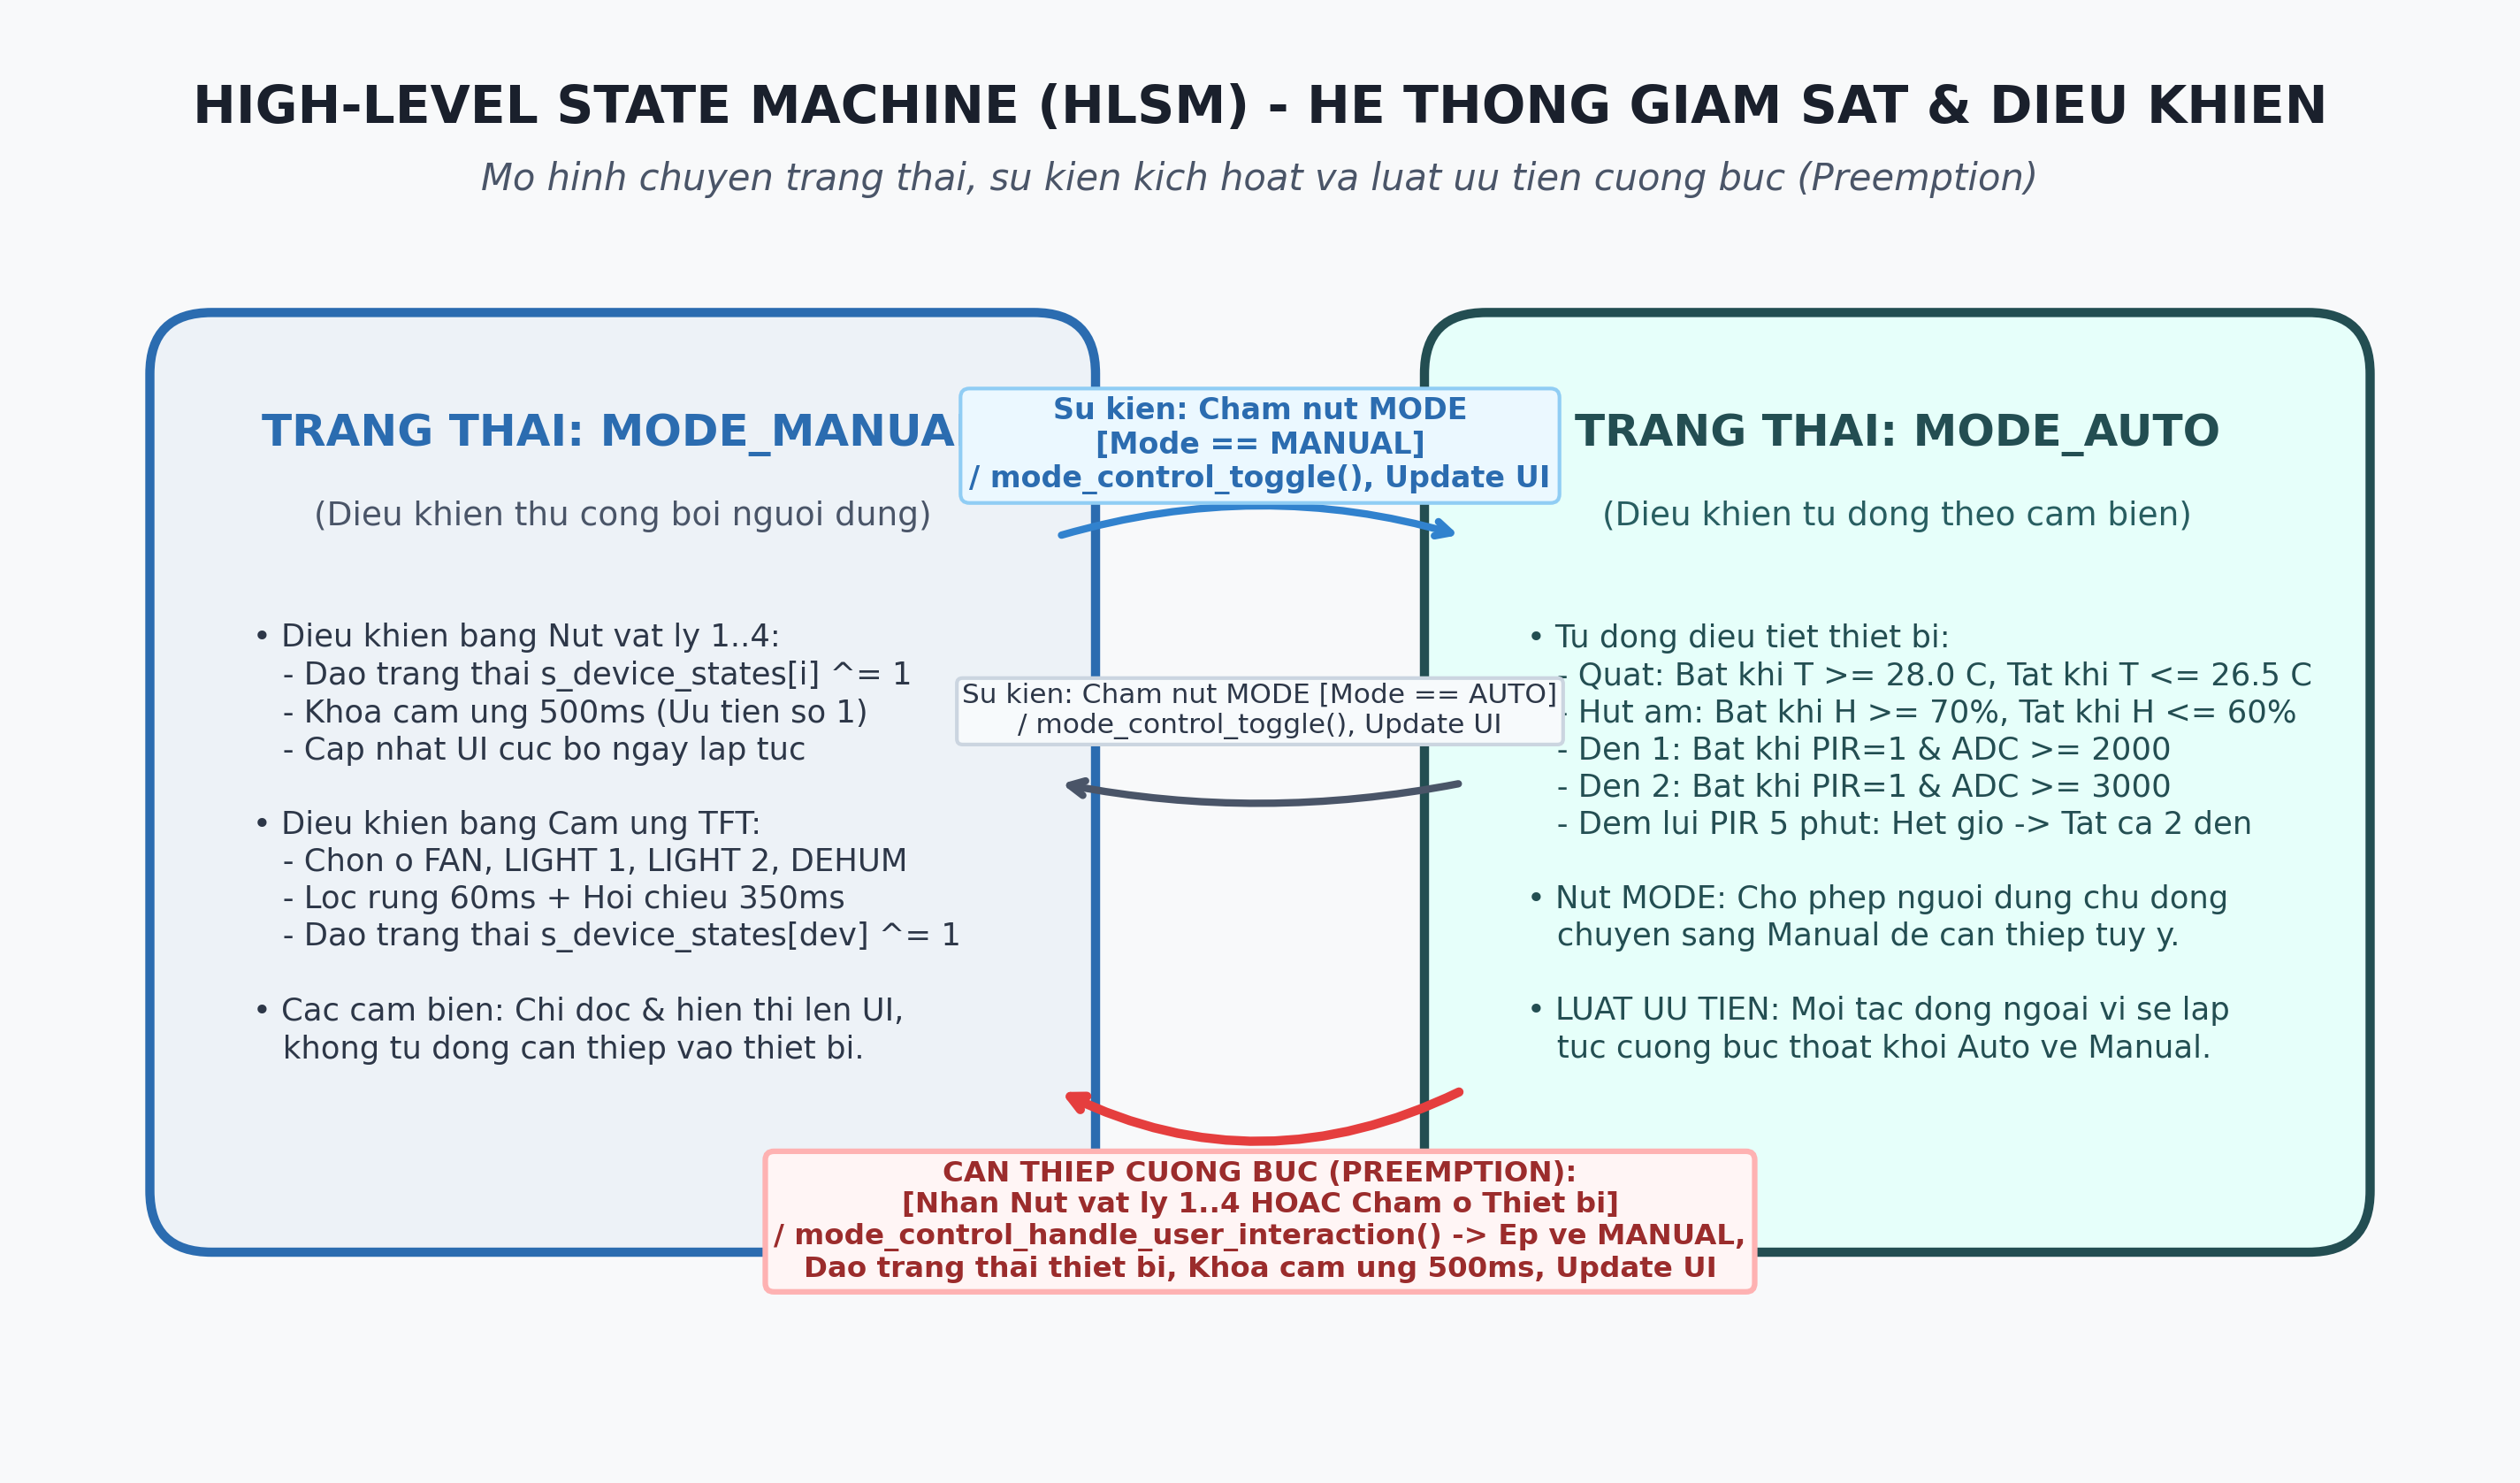
\includegraphics[width=0.95\textwidth]{figures/hlsm_system_mode.png}
    \caption{Máy trạng thái mức cao (HLSM) điều phối chế độ hoạt động}
    \label{fig:hlsm}
\end{figure}

\subsection{Các quy tắc chuyển đổi trạng thái cốt lõi}
\begin{enumerate}
    \item \textbf{Chuyển đổi chủ động (Normal Transition):} Khi người dùng chạm nút \texttt{MODE} trên màn hình TFT, hàm \texttt{mode\_control\_toggle()} được gọi để đảo trạng thái giữa \texttt{MANUAL} và \texttt{AUTO}.
    \item \textbf{Can thiệp cưỡng bức (Preemption Override):} Khi hệ thống đang ở \texttt{AUTO}, nếu có \textbf{bất kỳ tương tác nào} từ người dùng (nhấn 1 trong 4 nút vật lý hoặc chạm vào 1 trong 4 ô thiết bị trên màn hình), hệ thống lập tức cưỡng bức thoát khỏi \texttt{AUTO} và chuyển sang \texttt{MANUAL} thông qua hàm \texttt{mode\_control\_handle\_user\_interaction()}. Điều này đảm bảo an toàn tối đa và quyền kiểm soát tuyệt đối của con người.
\end{enumerate}

\section{Lưu đồ giải thuật Định thời Non-blocking (Cooperative Scheduler)}
Để tránh việc CPU bị "nghẽn" bởi các hàm trễ thô sơ \texttt{HAL\_Delay()}, chương trình áp dụng kỹ thuật \textbf{Cooperative Time-sliced Scheduler} dựa trên phép trừ không dấu của biến đếm thời gian hệ thống (\texttt{SysTick}):

\begin{figure}[H]
    \centering
    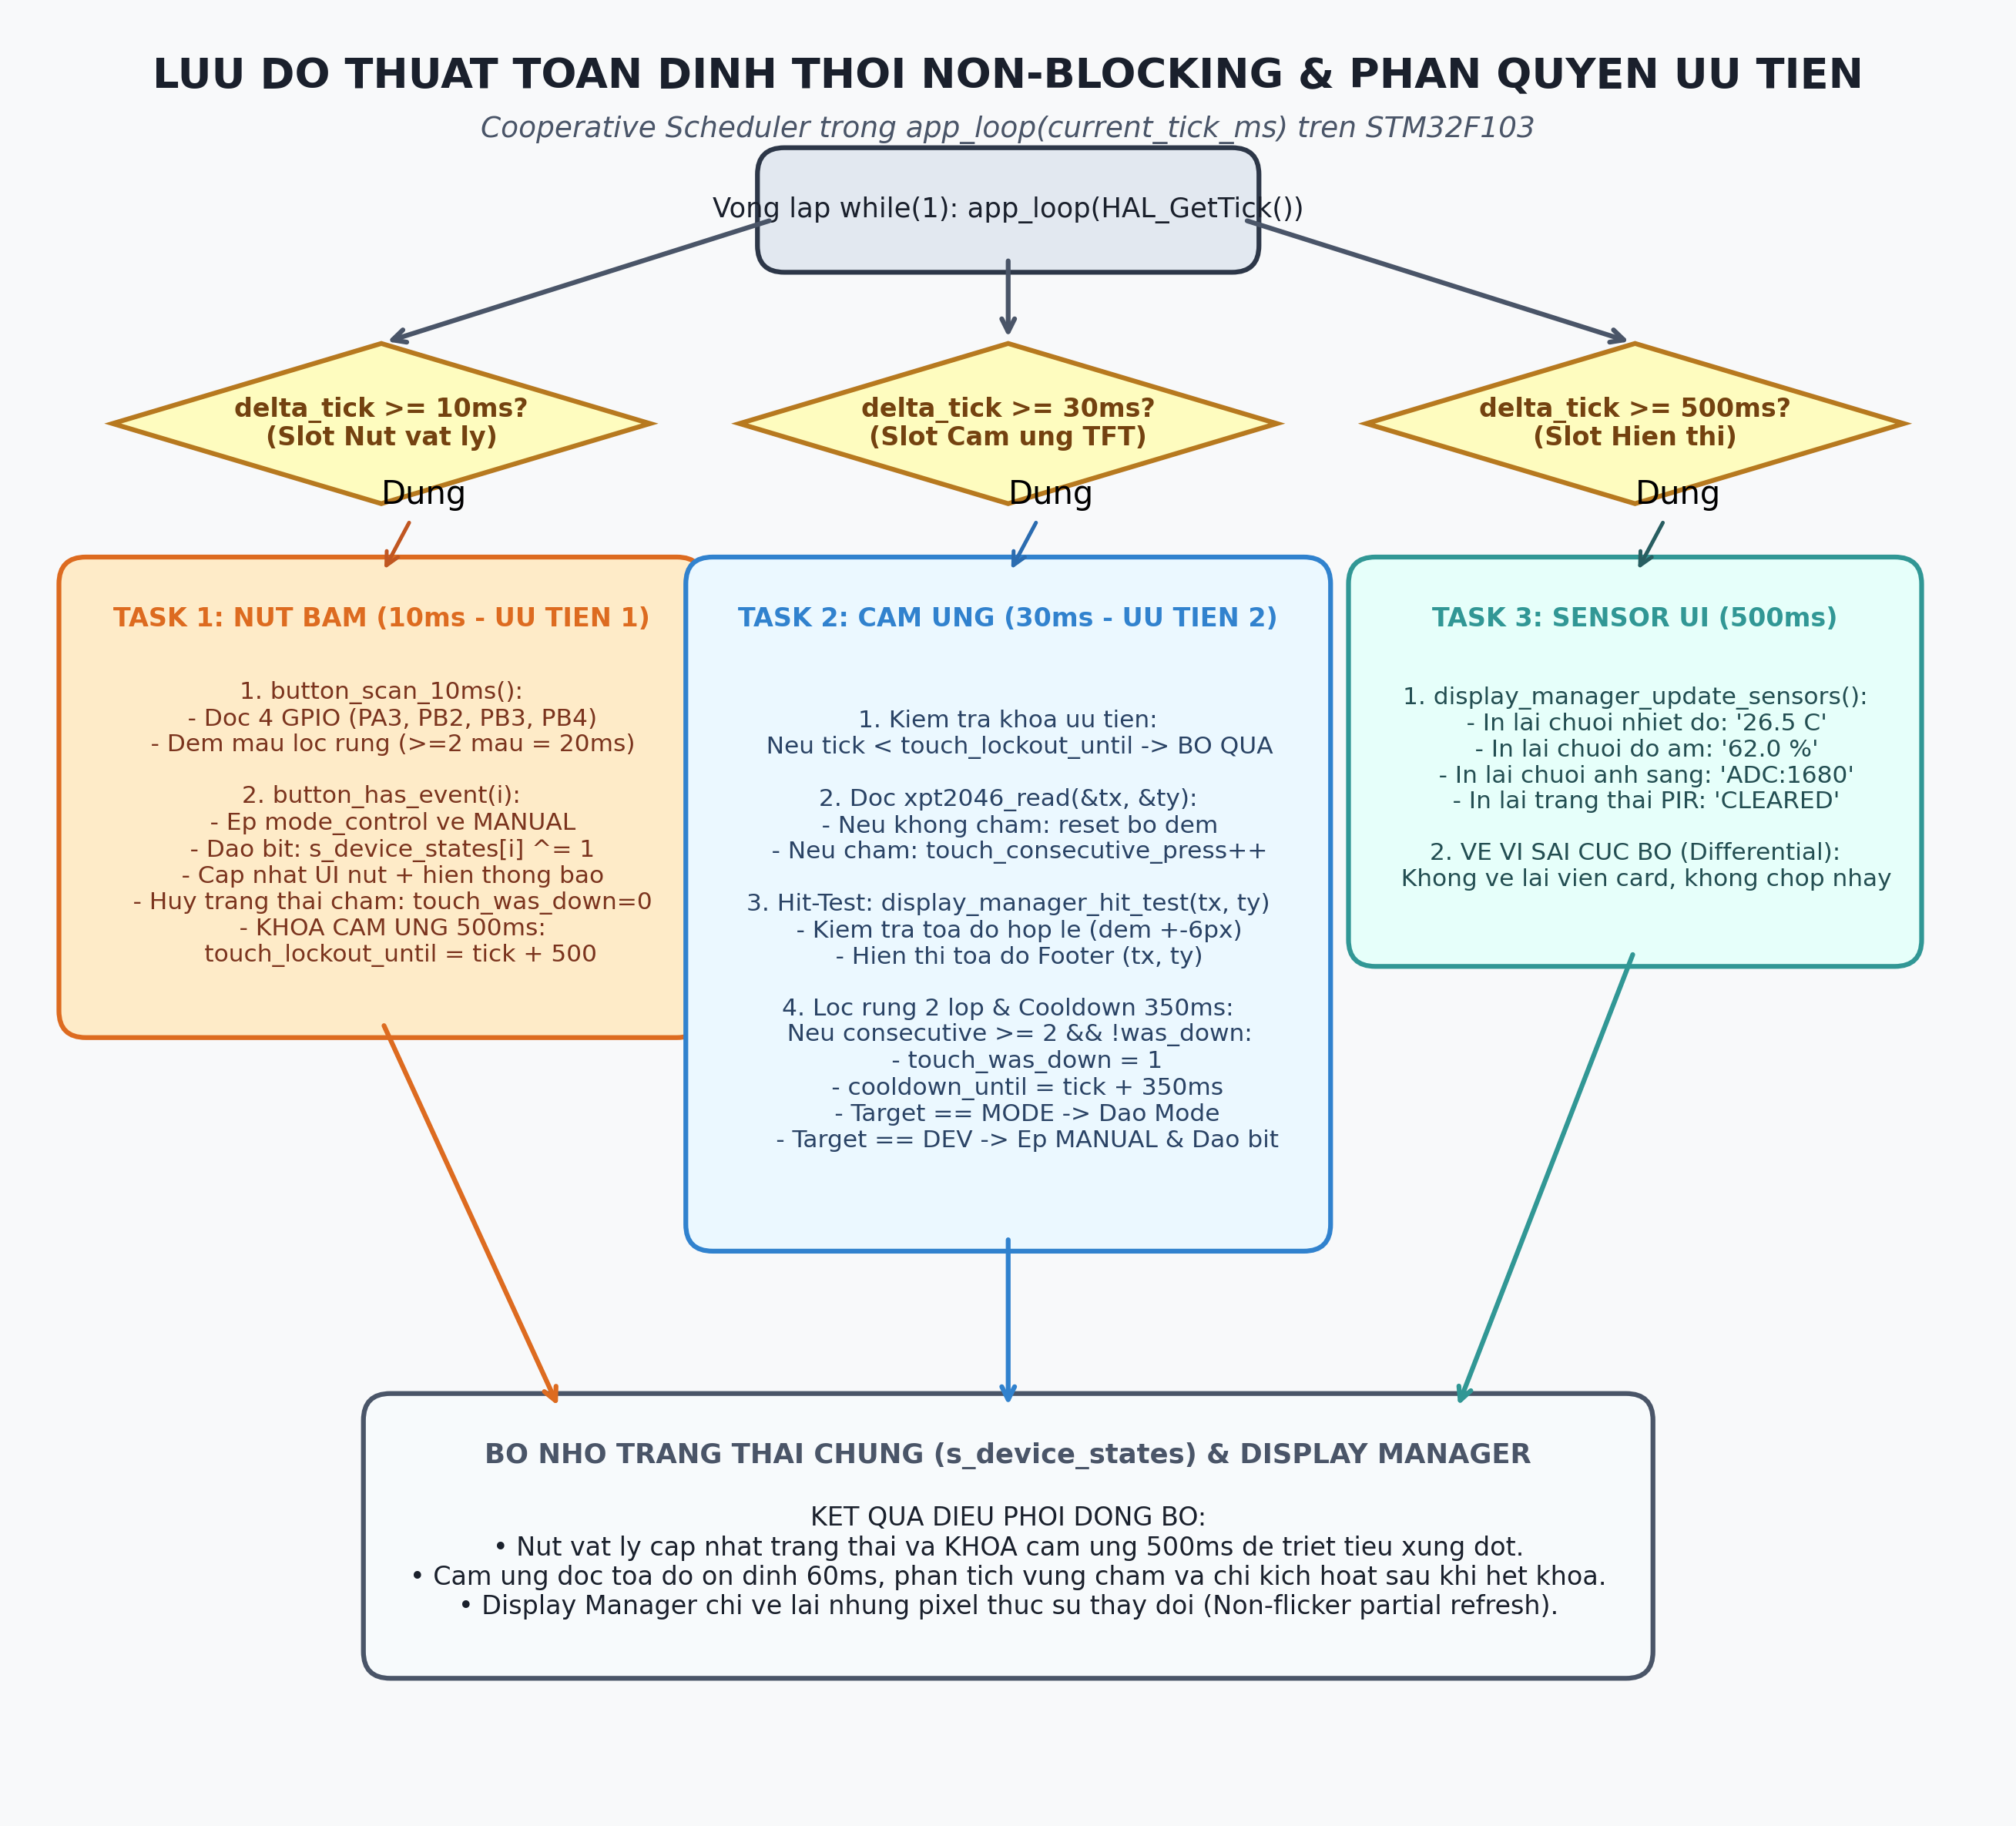
\includegraphics[width=0.88\textwidth]{figures/flowchart_scheduler.png}
    \caption{Lưu đồ giải thuật bộ điều phối thời gian Non-blocking và phân quyền ưu tiên}
    \label{fig:flowchart}
\end{figure}

\subsection{Ba rãnh thời gian độc lập và luật ưu tiên}
\begin{itemize}
    \item \textbf{Rãnh 1 - Quét nút vật lý (Chu kỳ 10ms - Ưu tiên cao nhất):} Quét 4 chân GPIO, đếm mẫu ổn định 2 chu kỳ ($20\text{ms}$) để lọc rung tiếp điểm cơ khí. Khi phát hiện nút nhấn hợp lệ:
    \begin{itemize}
        \item Đảo trạng thái thiết bị tương ứng: \texttt{s\_device\_states[i] \^{}= 1}.
        \item Hủy bỏ trạng thái cảm ứng dở dang (\texttt{touch\_was\_down = 0}).
        \item \textbf{Kích hoạt khóa cảm ứng 500ms:} \texttt{touch\_lockout\_until = current\_tick\_ms + 500}. Mọi tác động cảm ứng trong thời gian này đều bị bỏ qua để ngăn ngừa chạm nhầm khi đang thao tác nút vật lý.
    \end{itemize}
    \item \textbf{Rãnh 2 - Quét cảm ứng TFT (Chu kỳ 30ms - Ưu tiên thấp hơn):} 
    \begin{itemize}
        \item Kiểm tra cửa sổ khóa cảm ứng (\texttt{touch\_lockout\_until}).
        \item Lấy mẫu tọa độ XPT2046: Yêu cầu lấy mẫu ổn định liên tiếp 2 chu kỳ ($60\text{ms}$) để triệt tiêu nhiễu màng điện trở.
        \item Cửa sổ hồi chiêu 350ms (\texttt{touch\_cooldown\_until}): Ngăn chặn triệt để hiện tượng nảy tiếp điểm làm thiết bị bật/tắt liên tục trong một cú chạm.
        \item Thuật toán \textbf{Hit-Testing}: Dùng hàm \texttt{is\_inside()} với biên đệm $+6\text{px}$ để nhận diện vùng chạm chính xác.
    \end{itemize}
    \item \textbf{Rãnh 3 - Cập nhật hiển thị (Chu kỳ 500ms):} Làm mới thông số cảm biến môi trường.
\end{itemize}

\section{Kỹ thuật Hiển thị Vi sai Cục bộ (Differential Partial Redraw)}
Màn hình TFT ILI9341 giao tiếp qua bus SPI với băng thông giới hạn. Nếu vẽ lại toàn bộ màn hình ($320 \times 240 \times 2\text{ byte} = 153.6\text{ KB}$), màn hình sẽ bị giật và nhấp nháy liên tục (flicker). Giải pháp áp dụng trong mã nguồn:
\begin{itemize}
    \item Hàm \texttt{display\_manager\_draw\_screen()} chỉ chạy \textbf{1 lần duy nhất} khi khởi động để vẽ khung nền tĩnh.
    \item Khi nút thiết bị đổi trạng thái: Hàm \texttt{display\_manager\_update\_device()} chỉ định vị và tô lại đúng ô chữ nhật của nút đó (thời gian vẽ $< 1\text{ms}$).
    \item Khi cảm biến có số đo mới: Hàm \texttt{display\_manager\_update\_sensors()} chỉ vẽ đè chuỗi ký tự mới lên vùng giá trị, giữ nguyên viền khung của các thẻ Card.
\end{itemize}

\section{Bảng Tổng hợp Ngưỡng Kích hoạt Relay ở Chế độ Auto}
Bảng thông số vận hành tự động theo đặc tả hệ thống có tính toán trễ Hysteresis chống rung cơ khí:

\begin{table}[H]
\centering
\small
\begin{tabular}{@{}lllll@{}}
\toprule
\textbf{Thiết bị \& Kênh Relay} & \textbf{Cảm biến} & \textbf{Ngưỡng BẬT (ON)} & \textbf{Ngưỡng TẮT (OFF)} & \textbf{Độ trễ (Hysteresis)} \\ \midrule
\textbf{Quạt (Fan - PB5)} & DHT22 ($T$) & $\ge 28.0^\circ\text{C}$ & $\le 26.5^\circ\text{C}$ & $1.5^\circ\text{C}$ hysteresis \\
\textbf{Hút ẩm (Dehum - PB8)} & DHT22 ($H$) & $\ge 70.0\%$ & $\le 60.0\%$ & $10.0\%$ hysteresis \\
\textbf{Đèn 1 (Light 1 - PB6)} & PIR + LDR & PIR=1 \& ADC $\ge 2000$ & Hết 5 phút PIR hoặc ADC $\le 1700$ & 300 count hysteresis \\
\textbf{Đèn 2 (Light 2 - PB7)} & PIR + LDR & PIR=1 \& ADC $\ge 3000$ & Hết 5 phút PIR hoặc ADC $\le 2700$ & 300 count hysteresis \\ \bottomrule
\end{tabular}
\caption{Bảng ngưỡng kỹ thuật kích hoạt tải trong Auto Mode}
\label{tab:thresholds}
\end{table}

\end{document}
